One of the most fundamental problems in robotics is the Simultaneous Localization And Mapping problem (SLAM).
This problem arises when the robot does not have access to a map of the environment and does not know its own pose. 
This knowledge is critical for robots to operate autonomously.
SLAM is an active research area in robotics.
A variety of solutions have been developed.
Most solutions rely on bulky sensors that have a high range and accuracy (e.g., SICK laser range finder).
However, these bulky sensors cannot be used on small (flying) vehicles.
As a result, researchers focused on using vision sensors, which offer a good balance in terms of weight, accuracy and power consumption.
Lightweight cameras are especially attractive for small flying vehicles (AUVs).

Almost all publication related to my research describe a methodology that is able to learn the environment, but do not produce a visual map.
An exception is the research by Steder, which builds a visual map of the environment.


\begin{comment}
Building maps with robots equipped with perspective cameras has received increasing attention in the last decade. Davison et al. [7] proposed a single-camera SLAM algorithm based on a Kalman filter. The features considered in this approach are initialized by using a particle filter that estimates their depth. Civera et al. [5] extended this framework by proposing an inverse-depth parameterization of the landmarks. Since this parameterization can be accurately approximated by a Gaussian, the particle filter can be avoided in the initialization of the features. Subsequently, Clemente et al. [6] integrated this technique in a hierarchical SLAM framework, which has been reported to successfully build large-scale maps with comparably poor sensors.
Chekhlov et al. [3] proposed an online visual SLAM framework that uses a scale-invariant feature transform (SIFT)-like feature descriptors and tracks the 3-D motion of a single camera by using an unscented Kalman filter. The computation of the features is speeded up by utiliz- ing the estimated camera position to guess the scale. Jensfelt et al. [11] proposed an effective way for online mapping applications by combin- ing a SIFT feature extractor with an interest points tracker. While the feature extraction can be performed at low frequency, the movement of the robot is constantly estimated by tracking the interest points at high frequency.
\end{comment}

\section{Visual-map SLAM}

\subsubsection{Visual SLAM for flying vehicles}
The approach presented in this thesis was inspired by Steder \textit{et al.} \cite{steder2008visual}, who presented a system to learn large visual maps of the ground using flying vehicles.
The setup used is comparable to the AR.Drone, with an inertial sensor and a low-quality camera pointing downward.
If a stereo camera setup is available, their system is able to learn visual elevation maps of the ground.
If only one camera is carried by the vehicle, the system provides a visual map without elevation information.
Steder uses a graph-based formulation of the SLAM problem, in which the poses of the vehicle are described by the nodes of a graph.
Every time a new image is acquired, the current pose of the camera is computed based on both visual odometry and place revisiting.
The corresponding node is augment the graph accordingly.
Edges between these nodes represent spatial constraints between them.
The constructed graph serves as input to the TORO-based network optimizer \cite{Grisetti2007iros}, which minimizes the error introduced by the constraints.
The graph is optimized if the computed poses are contradictory.

\begin{figure}[htb!]
  \begin{center}
    \subfigure[Map constructed by a blimp]{\label{steder_blimp}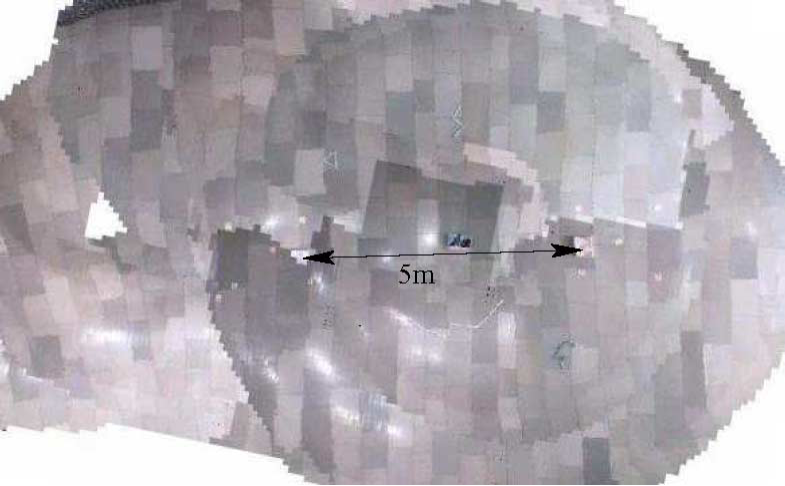
\includegraphics[height=3.5cm]{images/steder_blimp.png}}
    \hspace{1cm}
    \subfigure[Map constucted by a stereo camera platform. A sensor platform was mounted on a rod to simulate a freely floating vehicle.]{\label{steder_outdoor}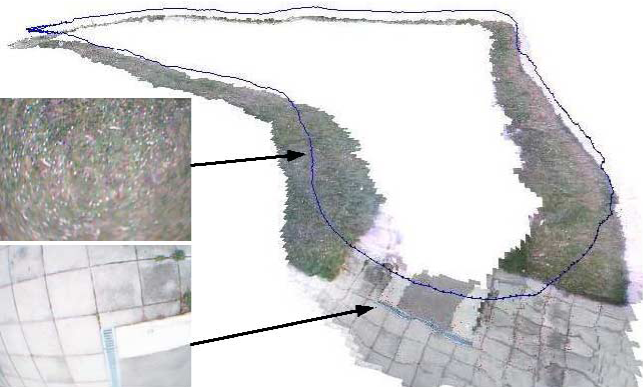
\includegraphics[height=3.5cm]{images/steder_outdoor.png}}
   
  \end{center}
  \caption{Visual maps obtained with the visual SLAM system presented in \cite{steder2008visual}.}
  \label{featureImg}
\end{figure}

Each node models a 6 degree of freedom camera pose.
The spatial constraints between two poses are computed from the camera images and the inertia measurements.
%The camera images are used to estimate the relative motion of the camera.
To do so, visual features are extracted from the images obtained from downlooking cameras.
Steder uses Speeded-Up Robust Features (SURF) \cite{Bay2008cviu} that are invariant with respect to rotation and scale.
By matching features in current image to the ones stored in the previous $n$ nodes, one can estimate the relative motion of the camera (\textit{visual odometry}).
The inertia sensor provides the roll and pitch angle of the camera.
This reduces the dimensionality of each pose that needs to be estimated from $\R^6$ to $\R^4$.
For each node, the observed features as well as their 3D positions relative to the node are stored.
The constraints between nodes are computed from the features associated with the nodes.

In the case of place revisiting, they compare the features of the current frame with all previous featured.
To speed up this potentially expensive operation, multiple filters are used.
First, only the features from robot poses that lie within Tipaldi's \cite{tipaldi2007approximate} confidence interval are used.
Second, only the best features from the current image are used (i.e., features with the lowest descriptor distance during visual odmetry).
Finally, a $k$-D tree is used to efficiently query for similar features, together with the best-bins-first technique proposed by Lowe \cite{lowe1999object}.

The camera pose is computed as following.
Using known camera calibration parameters, the positions of the features are projected on a normalized image plane.
Now, the altitude of the camera is computed by exploiting the similarity of triangles.
Once the altitude is known, the yaw of the camera is computed by projecting map features (from previous camera images) into the same normalized image plane.
When matching two features from the camera image against two features from the map, the yaw is the angle between the two  lines on this plane.
Finally, the feature positions from the camera image are projected into the map according to the known altitude and yaw angle.
The $x$ and $y$ coordinates are determined as the difference between the positions of the map features and the projections of the corresponding image points.

Both visual odometry and place revisiting return a set of correspondences, from which the the most likely camera transformation is computed.
First, these correspondences are ordered according to the Euclidean distance of their descriptor vectors, such that the best correspondences are used first.
The transformation $T_{c_a,c_b}$is determines for each correspondence pair.
This transformation is then evaluated based on the other features in both sets using a score function.
The score function calculates the relative displacement between the image features and the map features projected into the current camera image.
The solution with the highest score is returned as the assumption for the transformation.

Features correspondences between images are selected using a deterministic PROSAC \cite{chum2005matching} algorithm.
PROSAC takes into account a quality measure (e.g., distance between feature descriptors) of the correspondences during sampling, where RANSAC draws the samples uniformly.

This article describes how to estimate the motion of a vehicle and perform place revisiting using a feature map.
However, the article doesn't describe how the visual map is constructed (from poses and images) and visualized.
Furthermore, it lacks how an elevation map is constructed and how this elevation map can be used to improve the position estimates (e.g., elevation constraints).
A great disadvantage of the described method are the computational costs of the optimization method, which cannot be performed online (i.e. during flight). This reduces the number of practical applications.


\subsubsection{Online Mosaicking}
While Steder uses a Euclidean distance measure to compare the correspondences of the features in two images, Caballero \textit{et al.} \cite{caballero2009unmanned} indicate that this is a last resort.
They are able to make a robust estimation of the spatial relationship on different levels: homogeneous, affine and Euclidean.
The article addresses the problem for aerial vehicles with a single camera, like the AR.Drone.
%Geo-referenced mosaics can be sufficient as environment model for certain tasks.
A mosaic is built by aliging a set of images gathered to a common frame, while the aerial vehicle is moving.
A set of matches between two views can be used to estimate a homographic model for the apparent image motion.

\begin{figure}[htb]
\centering
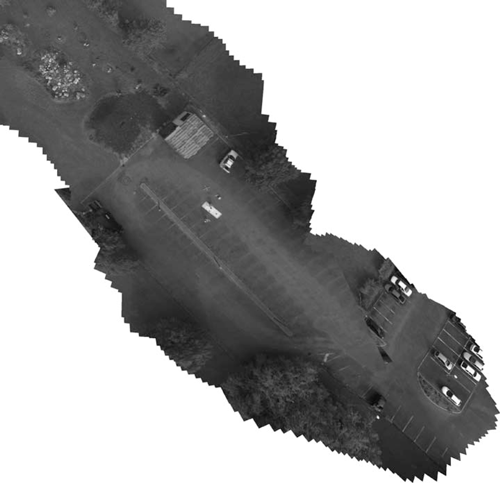
\includegraphics[width=6cm]{images/Caballero_map.png}
\caption{Mosaic constructed with a KARMA autonomous airship flying at $22\small{m}$.}
\label{fig:Caballero_map}
\end{figure}


The homography that relates two given images is computed from sets of matched features.
Depending on the scene characteristics (e.g., the parallax effect and small overlap between images), the homography computation could become a hard problem. 
A classical solution to improve the results is to introduce additional constraints to reduce the number of degrees of freedom of the system of equations.
This is accomplished through a hierarchy of homographic models, in which the complexity of the model to be fitted is decreased whenever the system of equations is ill-constrained.
An estimation of this accuracy will be given by the covariance matrix of the computed parameters.

If most of the matches are tracked successfully, a \textit{complete homogeneous transformation} (8 degrees of freedom) is estimated.
Least median of squares (LMedS) is used for outlier rejection and a M-Estimator  \cite{zhang1997parameter} to compute the final result.
When the number of correspondences is too low, an \textit{affine transformation} (6 degrees of freedom) is estimated.
LMedS is not used, given the reduction in the number of matches.
Instead, a relaxed M-Estimator (soft penalization) is carried out to compute the model.
Only when the features in the image are really noisy a \textit{Euclidean transformation} (4 degrees of freedom) is estimated.
The model is computed using least-squares.
If the selected hierarchy level is not constrained enough (e.g., the M-Estimator diverges by reaches the maximum number of iterations), the algorithm decreases the model complexity.
Once the homography is computed, it is necessary to obtain a measure of the estimation accuracy.
Caballero uses a $9 \times 9$ covariance matrix of the homography matrix, which is explained in \cite{hartley2000multiple}.

The (ego-) motion of the vehicle is computed using the estimated homographies.
This method assumes that the terrain is approximately flat and that cameras are calibrated.
$H_{12}$ is the homography that relates the first and the second view of the planar scene.
Both projections can be related to the camera motion as:
\begin{equation}
H_{12} = AR_{12}(I - \frac{t_2n_i^T}{d_1})A^{-1}
\end{equation}
where $A$ is the camera calibration matrix, $t_2$ is the relative translation of the second view, $n_1$ is an unitary vector normal to the plane in the first camera coordinate frame, $d_1$ is the distance from the first camera to the plane and $R_{12}$ is the rotation matrix that transforms a vector in the first camera coordinate frame into a vector expressed in the second camera coordinate frame.
If the camera calibration matrix $A$ and the distance to the ground $d_1$ are known, it is possible to extract the motion of the vehicle.
Triggs \cite{triggs1998autocalibration} proposes a robust algorithm based on the singular value decomposition of the calibrated homography, defined by:
\begin{equation}
H_{12}^{u} = A^{-1} H_{12} A
\end{equation}

A classical static mosaic is not appropriate, as the uncertainties should be taken into account along the mosaicking process.
Therefore, the mosaic is augmented by including stochastic information, resulting in a set of images linked by stochastic relations.

The position of the image inside the mosaic is obtained by multiplying the current homography by all the previous homographies.
This estimation will drift along time, but can be compensated by building a mosaic.
By comparing the current image with images previously stored in the mosaic, loop-closures can be detected and used to eliminate the accumulated drift.
The crossover detection consists of finding one image whose Mahalanobis distance is within a certain empirical range.
Once an image is detected, a feature matching is used to compute the alignment between both images. 
\textit{In the general case, the task of matching images taken from very different viewpoints is difficult and computationally costly.}
For this reason, the image is warped to match the image from the mosaic, which simplifies the problem.
The computed homography is used to obtain the correct alignment.
Now, the relations among the most recent image and the corresponding image from the mosaic can be updated.

The relations between images are maintained and updated by using an Extended Kalman Filter.
The state vector including the mean and covariance of all images is defined as:
\begin{equation}
x^{-} = [x_1, x_2, ..., x_n]^T = [h_{01}, x_1 \cdot h_{12}, ..., x_{(n-1)n} \cdot h_{(n-1)n}]^T
\end{equation}
The correction obtained when a loop-closing is detected is employed to update the state.
All states affected by the correct are now update by the Extended Kalman Filter.

Similar to Steder's research, Caballero uses a probabilistic representation of the estimated poses.
Both approaches optimize the map after a loop-closure event is detected, but use different optimization methods.
Unfortunately, these optimization methods are computationally expensive and difficult to perform while flying.
Steder exploits the information from the inertia sensor to reduce the complexity of pose estimation, without decreasing the accuracy (degree of freedom) of the estimated pose.



\section{Airborne elevation mapping with an ultrasound sensor}
Multiple techniques have been presented that successfully employ an airborne radar sensor for building elevation maps (e.g., \cite{foessel2000radar, weiß2006airborne}).
Due to its large footprint, a radar sensor cannot be mounted on small UAVs.
Unlike a radar sensor, an ultrasound sensor can be carried by a small UAV.
This sensor provides feedback for altitude stabilization and obstacle detection.
According to my knowledge, no publication addresses the problem of elevation mapping using a single airborne ultrasound sensor.
[seabed using side-scan sonar]


\section{Research using the AR.Drone}
Because the AR.Drone is a quite recent development, the number of studies based on this platform is limited.

\subsubsection{Autonomous corridor and staircase flights}

A recent publication is from Cornell University \cite{Bills2011icra}, where an AR.Drone is used to automatically navigate corridors and staircases based on visual clues.
Their method method first classifies the type of indoor environment (e.g., corridors, staircases, rooms and corners) then uses vision algorithms based on perspective cues to estimate the desired direction to fly.
This method require very little computational power and can be used by a controller directly without building a 3D model.

The type of environment is determined using two algorithms.
The first method uses GIST features \cite{oliva2001modeling} with a Support Vector Machine (SVM) learning algorithm for classification.
GIST features are well-suited for this task because they directly measure the global distribution of oriented line segments in an image, which takes advantage of the long lines found in indoor images.
The second method computes a confidence estimate from both the stair and corridor vision algorithms.
The confidence values are compared, and the highest is used to select the environment type.

When navigating corridors, vanishing points are used to locate the end of the corridor. 
First, the Canny edge detector is used to detected edges and a probabilistic Hough transform is used to find long lines.
The vanishing points (i.e., end of the corridor) are found by searching for the image region which has the highest density of pair-wise line intersections.
A probabilistic model with Gaussians is constructed to model the noise in the location of a vanishing point.
Staircases can be nagivated by finding the center of the staircase, so the AR.Drone can follow the staircase using its onboard intelligence (i.e., altitude stabilization).
Lines that represent the staircase are found by classifying the line segments as horizontal or vertical and looking for the largest horizontal-line cluster in the Hough transform space.
Once the cluster of horizontal lines is detected, the mean of the lines' endpoints is calculated to retrieve the desired direction.

\subsubsection{Map \& replay bearing-only navigation}
Krajn{\'\i}k et al \cite{krajník2010simple,faiglsurveillance} present a simple monocular navigation system based on the map-and-replay technique.
A robot is manually navigated through an environment and creates a map of its environment.
After that, the map is used for autonomous navigation.
The method can navigate a robot along a given path while observing only one landmark at a time, making it more robust than other monocular approaches.

At first, the robot is tele-operated in the environment along straight line segments in the mapping phase.
For each segment a set of visual landmarks is remembered, consisting of salient features detected in images captured by the robot’s forward- looking camera.
SURF features were used to detect and represent salient features.

After the mapping phase is completed, the AR.Drone is able to repeat the learned path.
During the navigation along a segment, the robot establishes correspondences of the currently seen and previously mapped landmarks and computes differences in the expected and recognized positions for each such correspondence.
The robot steers in a direction that reduces those differences while moving straight at a constant speed until its odometry indicates that the current segment has been traversed.

[how is the position estimated? IMU?]

The distance traveled along the segment is estimated purely by dead reckoning
Due to the low precision of the IMU based distance estimation, the localization error is high.
However, the localization error does not diverge and is kept within sufficient limits allowing the drone to autonomously navigate along the learned path.
